\documentclass[usletter]{article}
\usepackage{DejaVuSans}
\renewcommand*\familydefault{\sfdefault}
\usepackage[T1]{fontenc}
\usepackage{graphicx}
\usepackage{listings}
\lstset{
  breaklines=true,
  postbreak=\mbox{\textcolor{red}{$\hookrightarrow$}\space},
}
\usepackage{pdfpages}
\usepackage[hidelinks]{hyperref}
\begin{document}

  \begin{titlepage}
  \begin{center}

  {\Huge cocotbext uP}

  \vspace{25mm}

  \includegraphics[width=0.90\textwidth,height=\textheight,keepaspectratio]{img/AFRL.png}

  \vspace{25mm}

  \today

  \vspace{15mm}

  {\Large Jay Convertino}

  \end{center}
\end{titlepage}

\tableofcontents

\newpage

\section{Usage}

\subsection{Introduction}

\par
Cocotb extension to test uP bus master, and slave devices.

\subsection{Dependencies}

\par
The following are the dependencies of the cores.

\begin{itemize}
  \item iverilog (simulation)
  \item cocotb (simulation)
  \item cocotb-bus (simulation)
  \item cocotbext-busbase (simulation)
\end{itemize}

\subsection{In a Simulation}
\par
Below is a simple example for reading and writing data from register zero in the cocotb extension.
\begin{lstlisting}[language=Python]

master  = upMaster(dut, "apb", dut.clk, dut.rstn)
slave = upEchoSlave(dut, "apb", dut.clk, dut.rstn)

await master.write(0, 0xAAAAAAAA)

rx_data = await master.read(0)

assert 0xAAAAAAAA == rx_data, "RECEIVED DATA DOES NOT MATCH"

\end{lstlisting}

\section{Architecture}

Please see \ref{Code Documentation} for more information.

\par
upMaster tests uP slave devices by executing read/write requests from the python test bench.
\par
upEchoSlave provides a simple slave that will echo all register writes back over read when requested.
\par
upMonitor tests to make sure signals are proper. Simple core at the moment, only checks for 0 at rest
and if the wack/rack is correct per wreq/rreq.

\subsection{Directory Guide}

\par
Below highlights important folders from the root of the directory.

\begin{enumerate}
  \item \textbf{docs} Contains all documentation related to this project.
    \begin{itemize}
      \item \textbf{manual} Contains user manual and github page that are generated from the latex sources.
    \end{itemize}
  \item \textbf{cocotbext} Contains source files for the extension
    \begin{itemize}
      \item \textbf{up.ad} Contains source files for the Analog Devices uP version of the bus.
    \end{itemize}
  \item \textbf{tests} Contains test files for cocotb
\end{enumerate}

\newpage

\section{Simulation}
\par
A simulation for testing the cores can be run to verify operation.

\subsection{cocotb}
\par
To use the cocotb tests you must install the following python libraries.
\begin{lstlisting}[language=bash]
  $ pip install cocotb
  $ pip install -e .
\end{lstlisting}

Then you must enter the tests folder and enter the folder of the type you wish to test. From there you may execute the following command
which will kick off the test.
\begin{lstlisting}[language=bash]
  $ make
\end{lstlisting}

\newpage

\section{Code Documentation} \label{Code Documentation}

\par
Natural docs is used to generate documentation for this project. The next lists the following sections.

\begin{itemize}
  \item \textbf{init} Python init code.\\
  \item \textbf{monitor} Contains bus monitor code.\\
  \item \textbf{driver} Contains bus driver code.\\
  \item \textbf{absbus} Contains bus abstraction for monitor, and driver code.\\
  \item \textbf{busbase} Contains bus base for threads and read/write methods.\\
  \item \textbf{cocotb test} Python TestFactory code.\\
  \item \textbf{cocotb verilog test wrapper} Verilog wrapper module.\\
\end{itemize}



  %module documentation section

  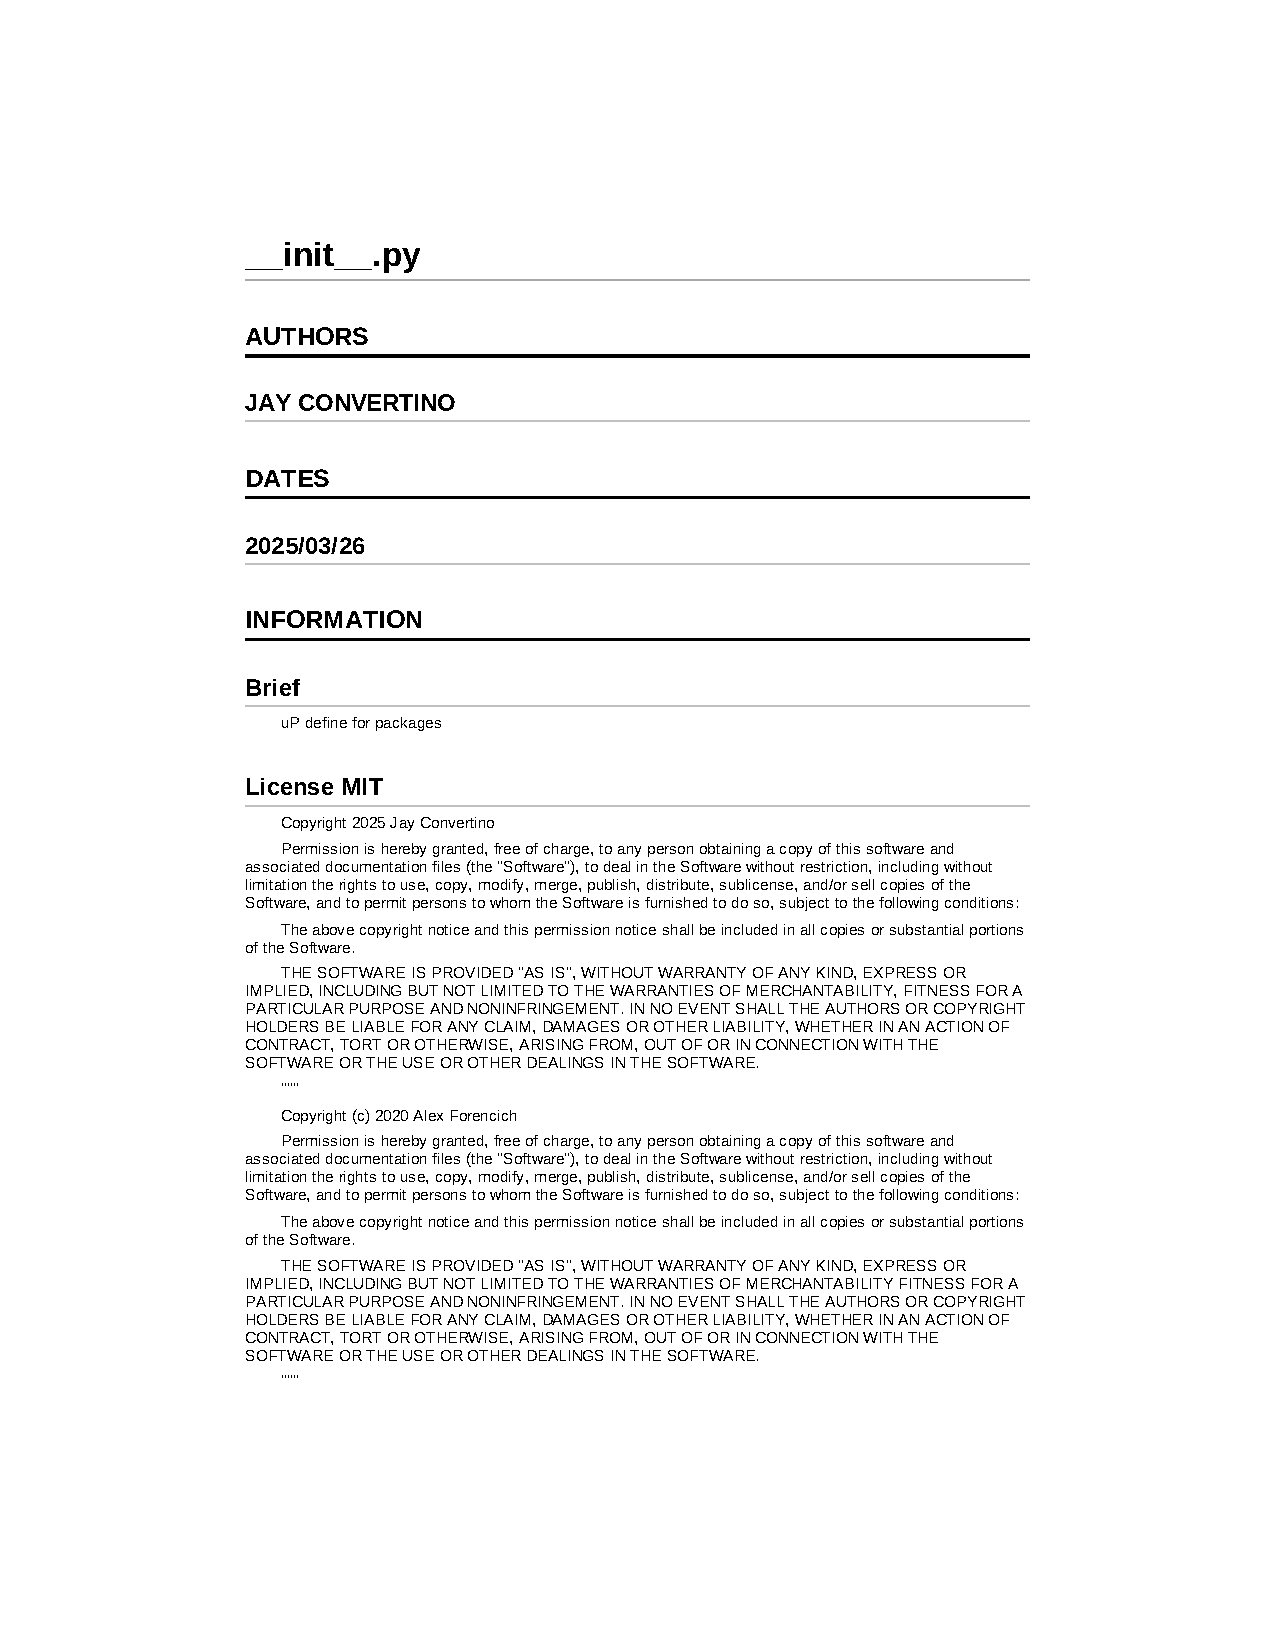
\includepdf[pages=-, addtotoc={1,subsection,1,init,p1}, pagecommand={}]{files___init__-py.pdf}
  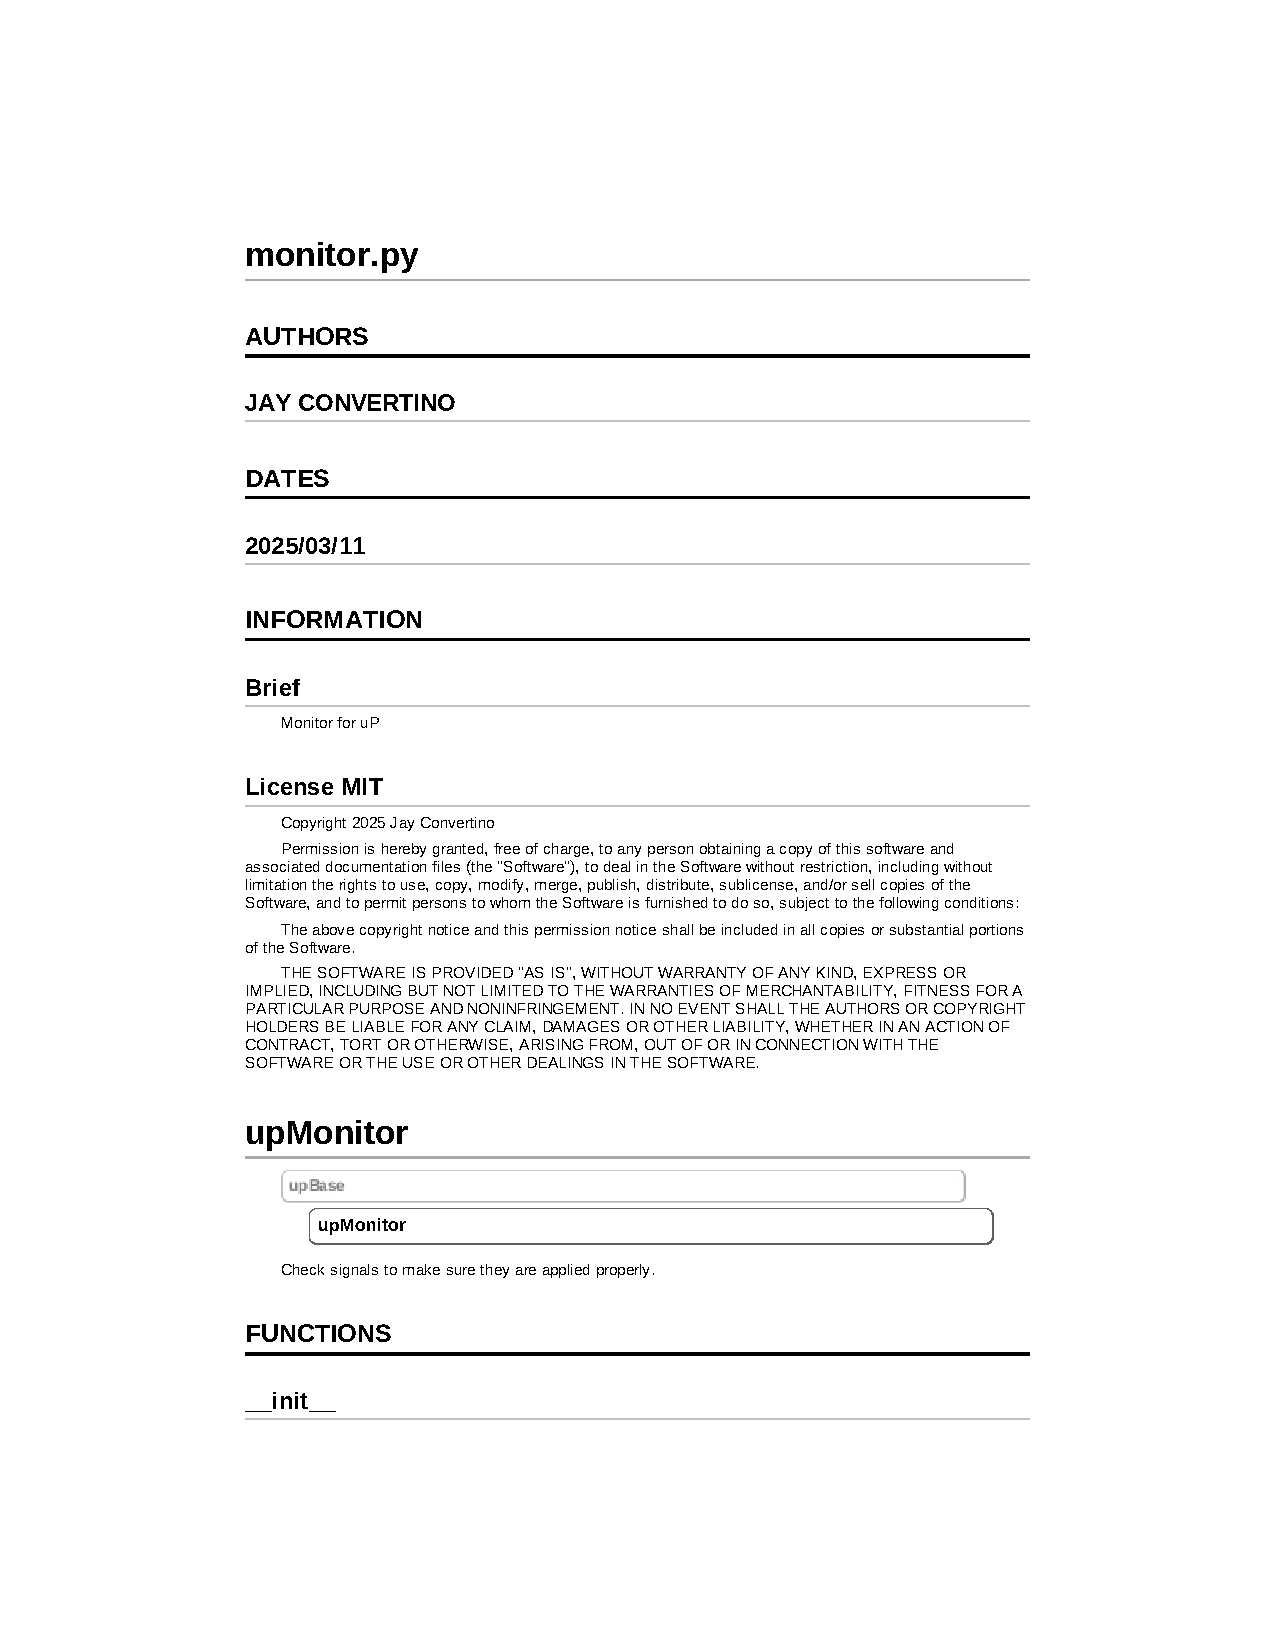
\includepdf[pages=-, addtotoc={1,subsection,1,monitor,p1}, pagecommand={}]{files_monitor-py.pdf}
  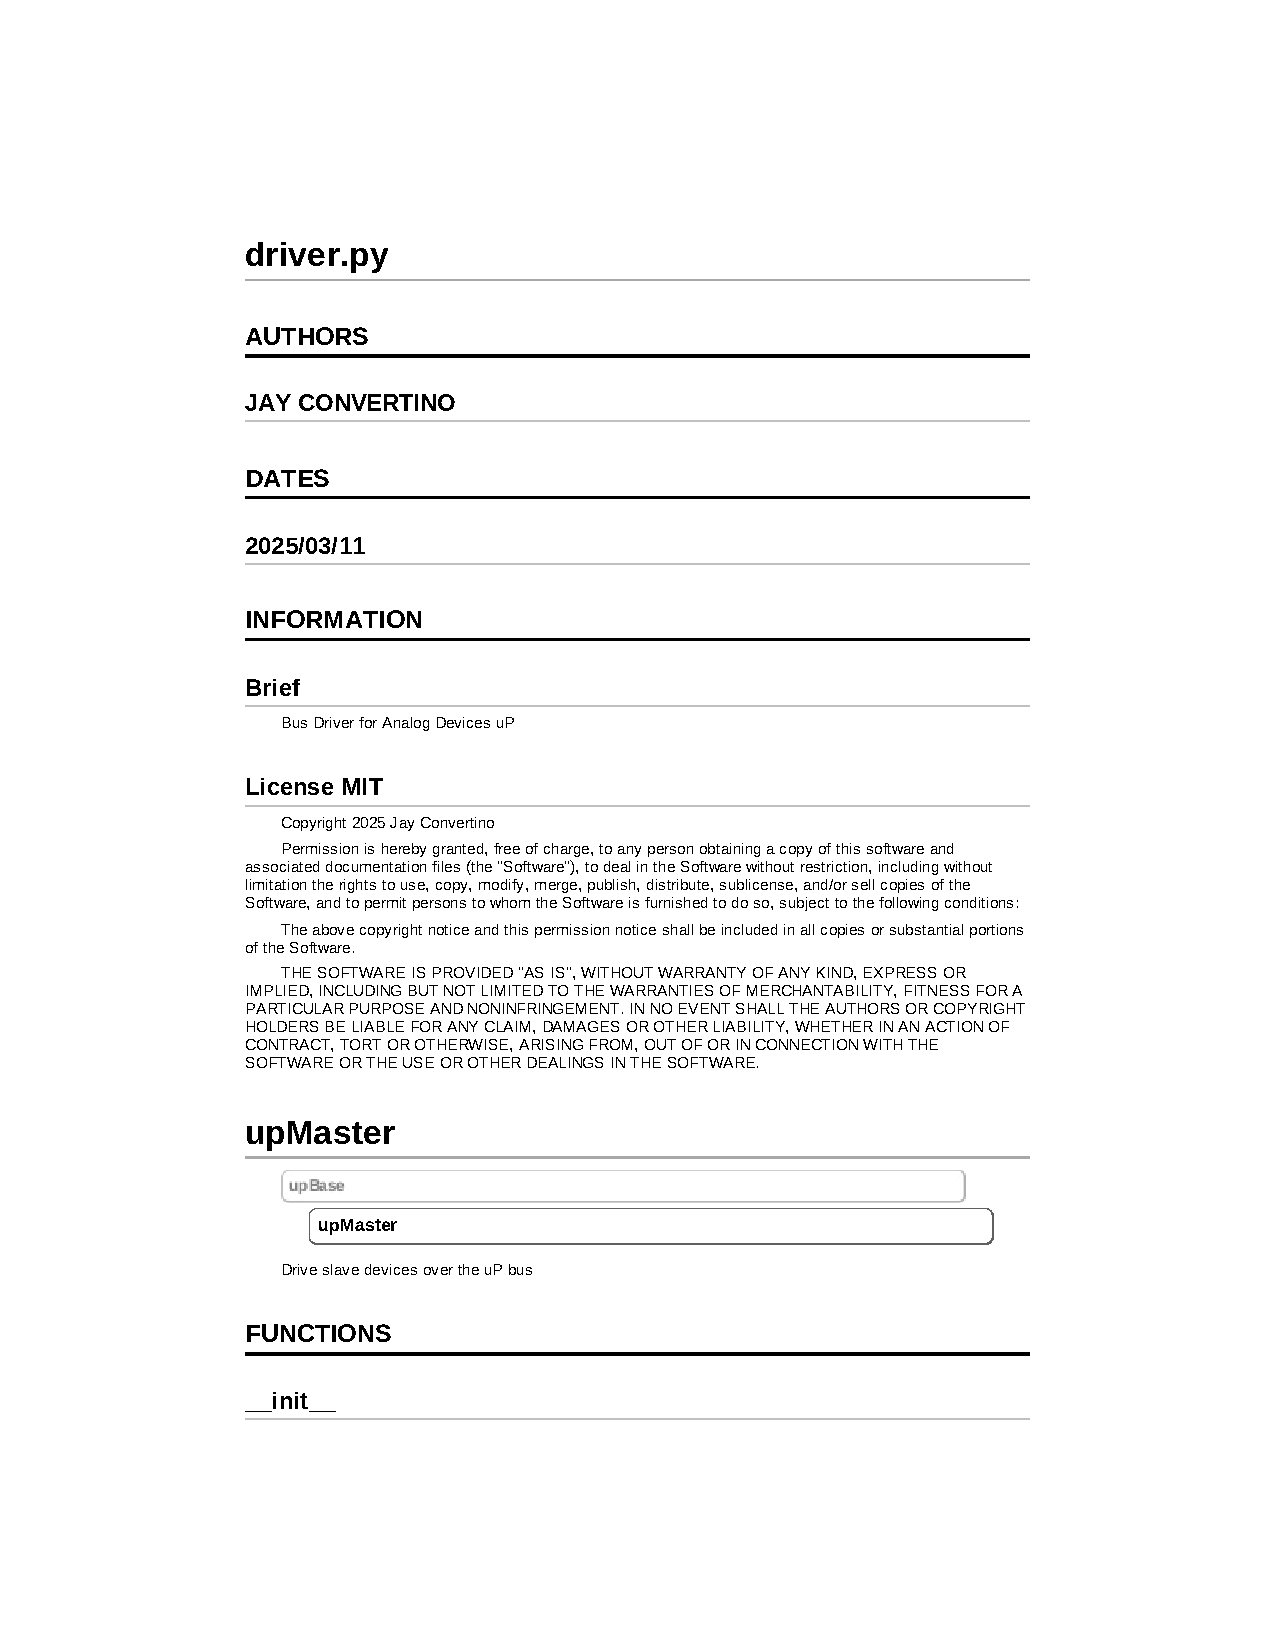
\includepdf[pages=-, addtotoc={1,subsection,1,driver,p1}, pagecommand={}]{files_driver-py.pdf}
  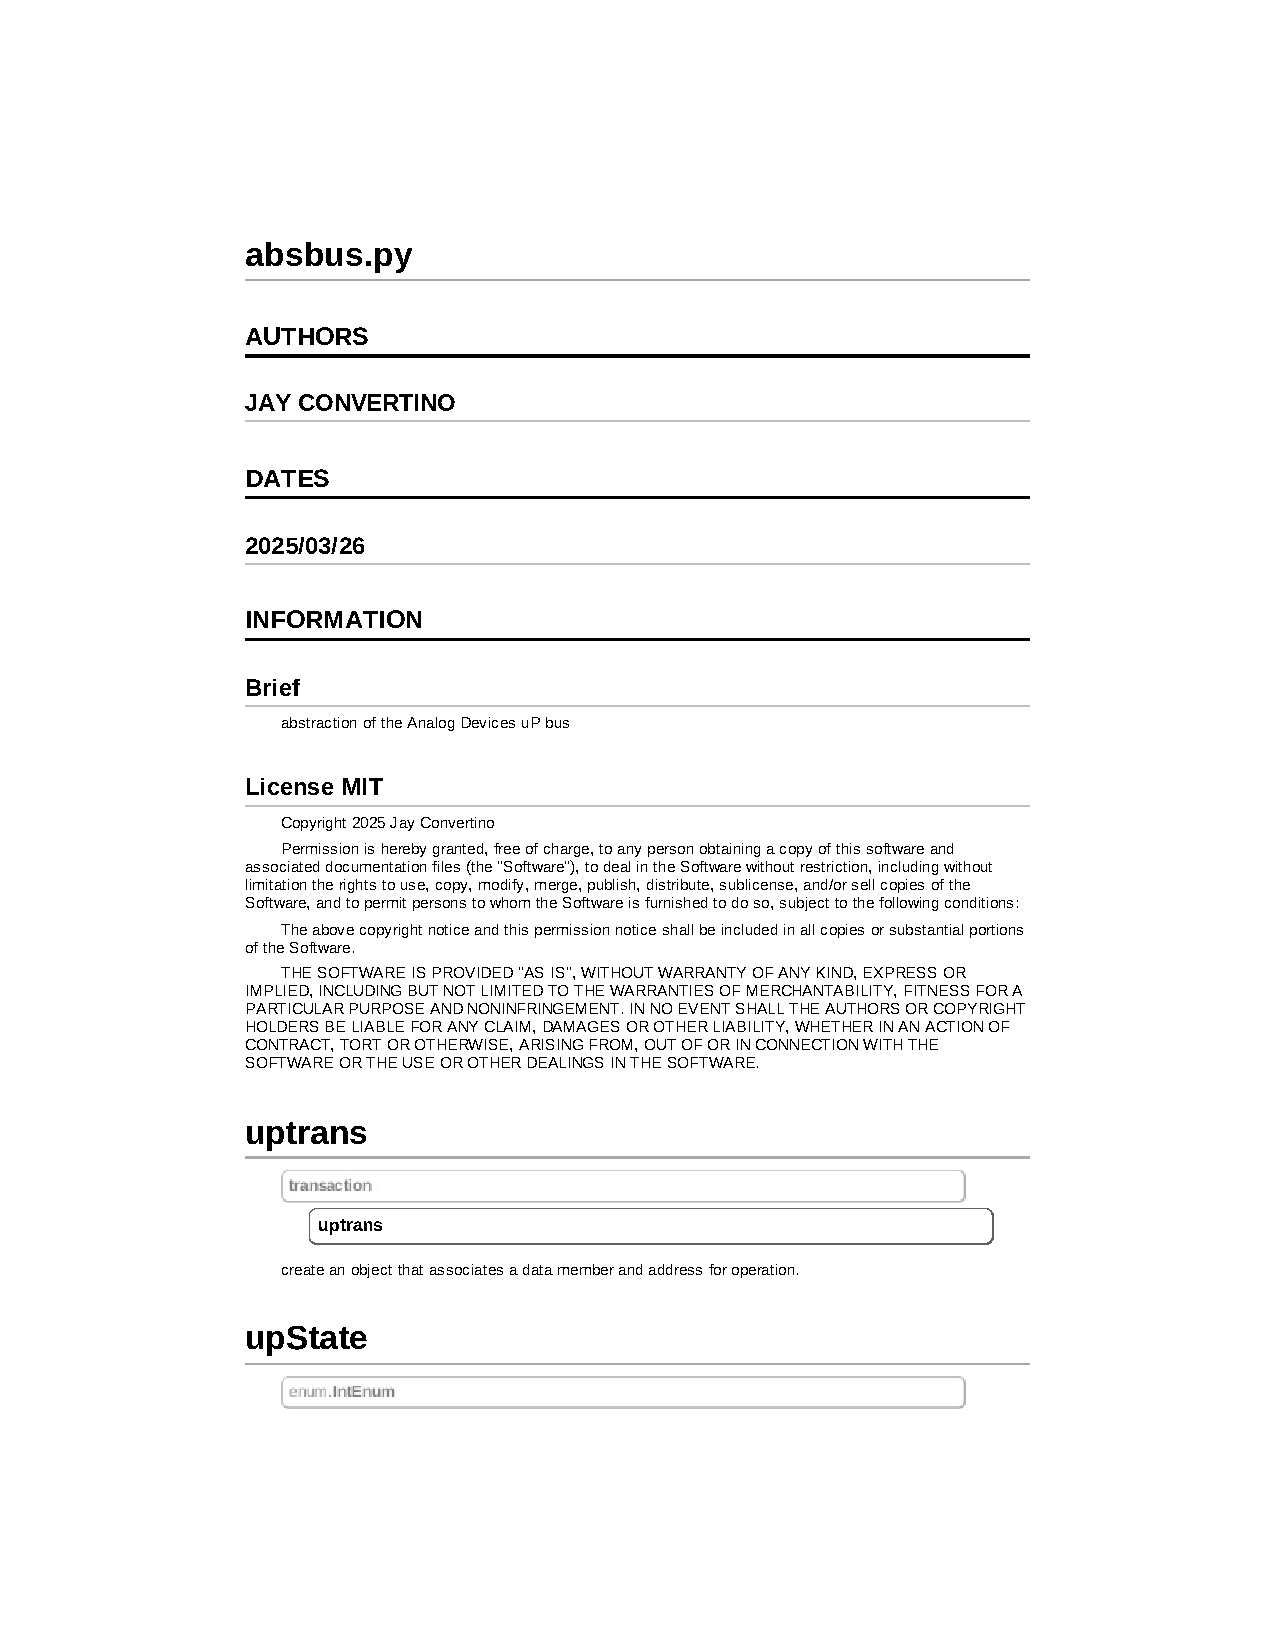
\includepdf[pages=-, addtotoc={1,subsection,1,absbus,p1}, pagecommand={}]{files_absbus-py.pdf}
  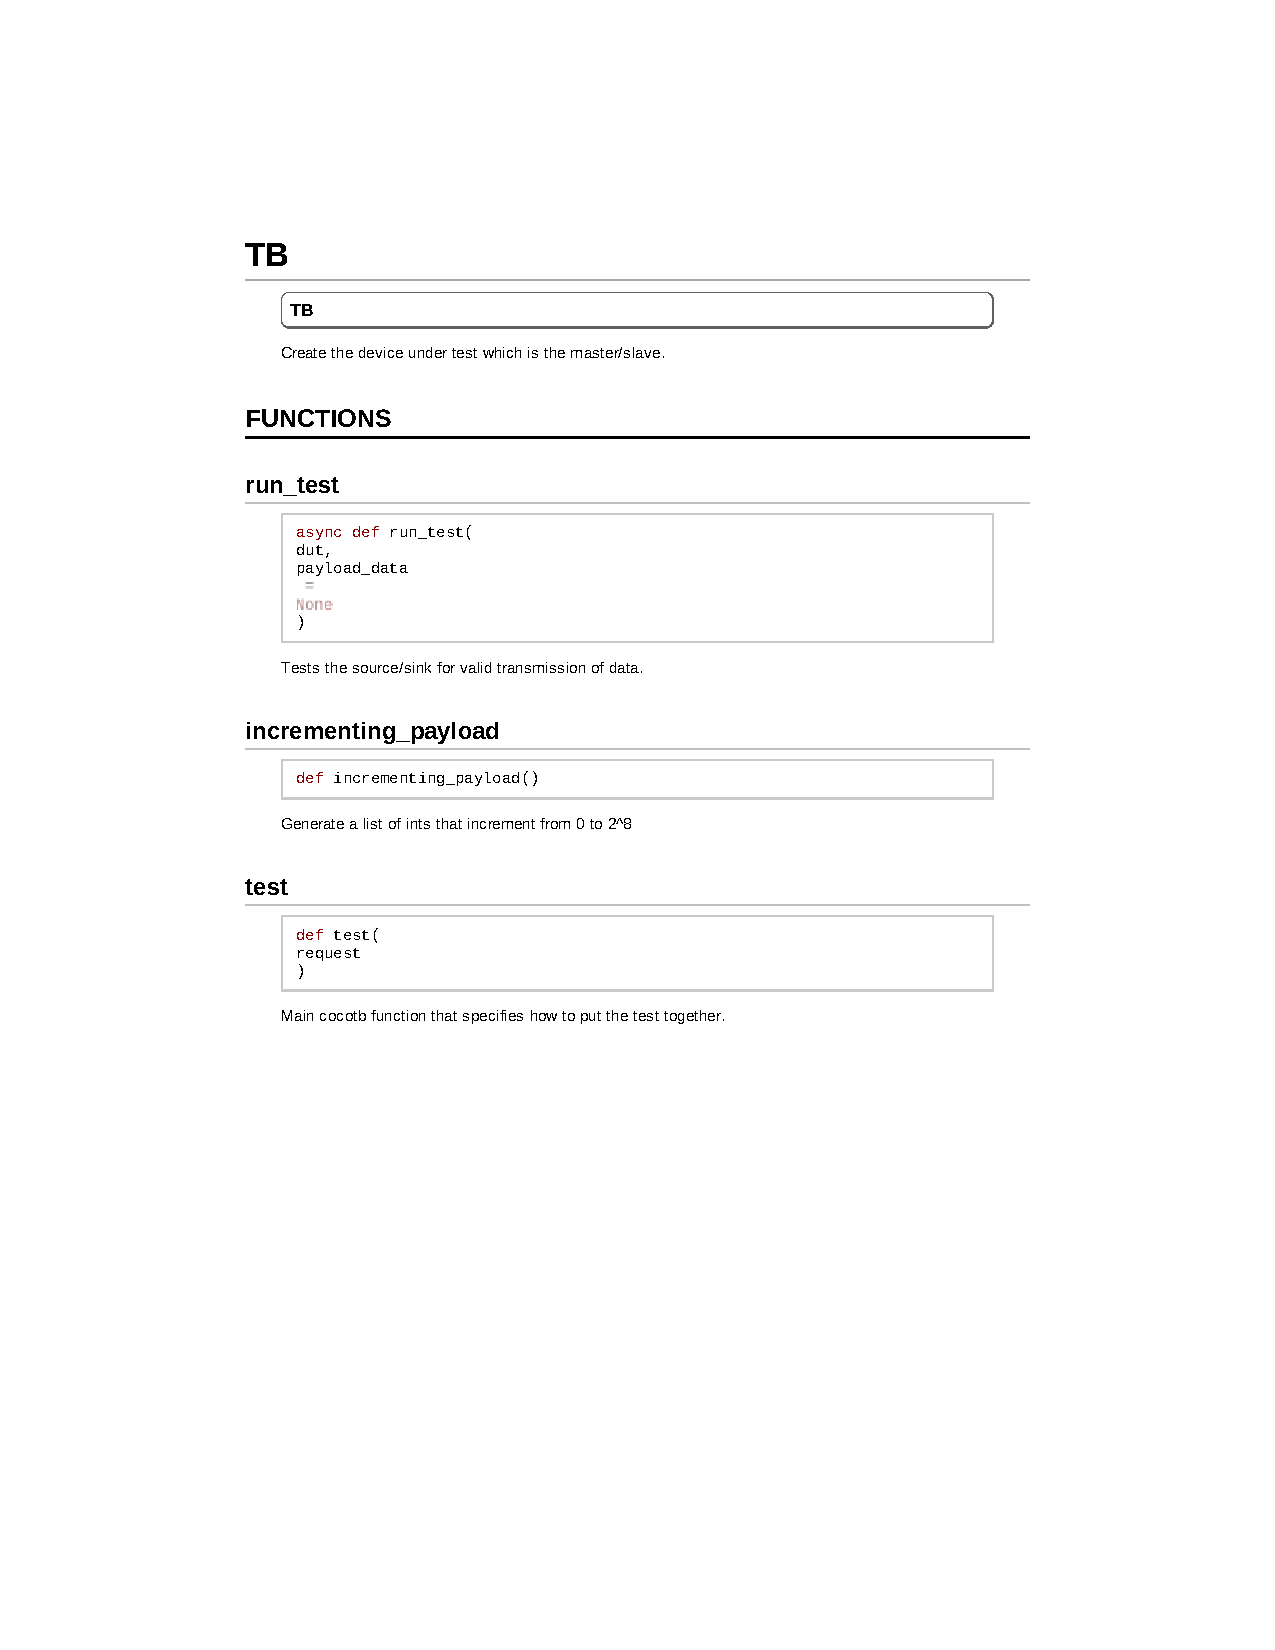
\includepdf[pages=-, addtotoc={1,subsection,1,test extension python,p1}, pagecommand={}]{files2_test-py.pdf}
  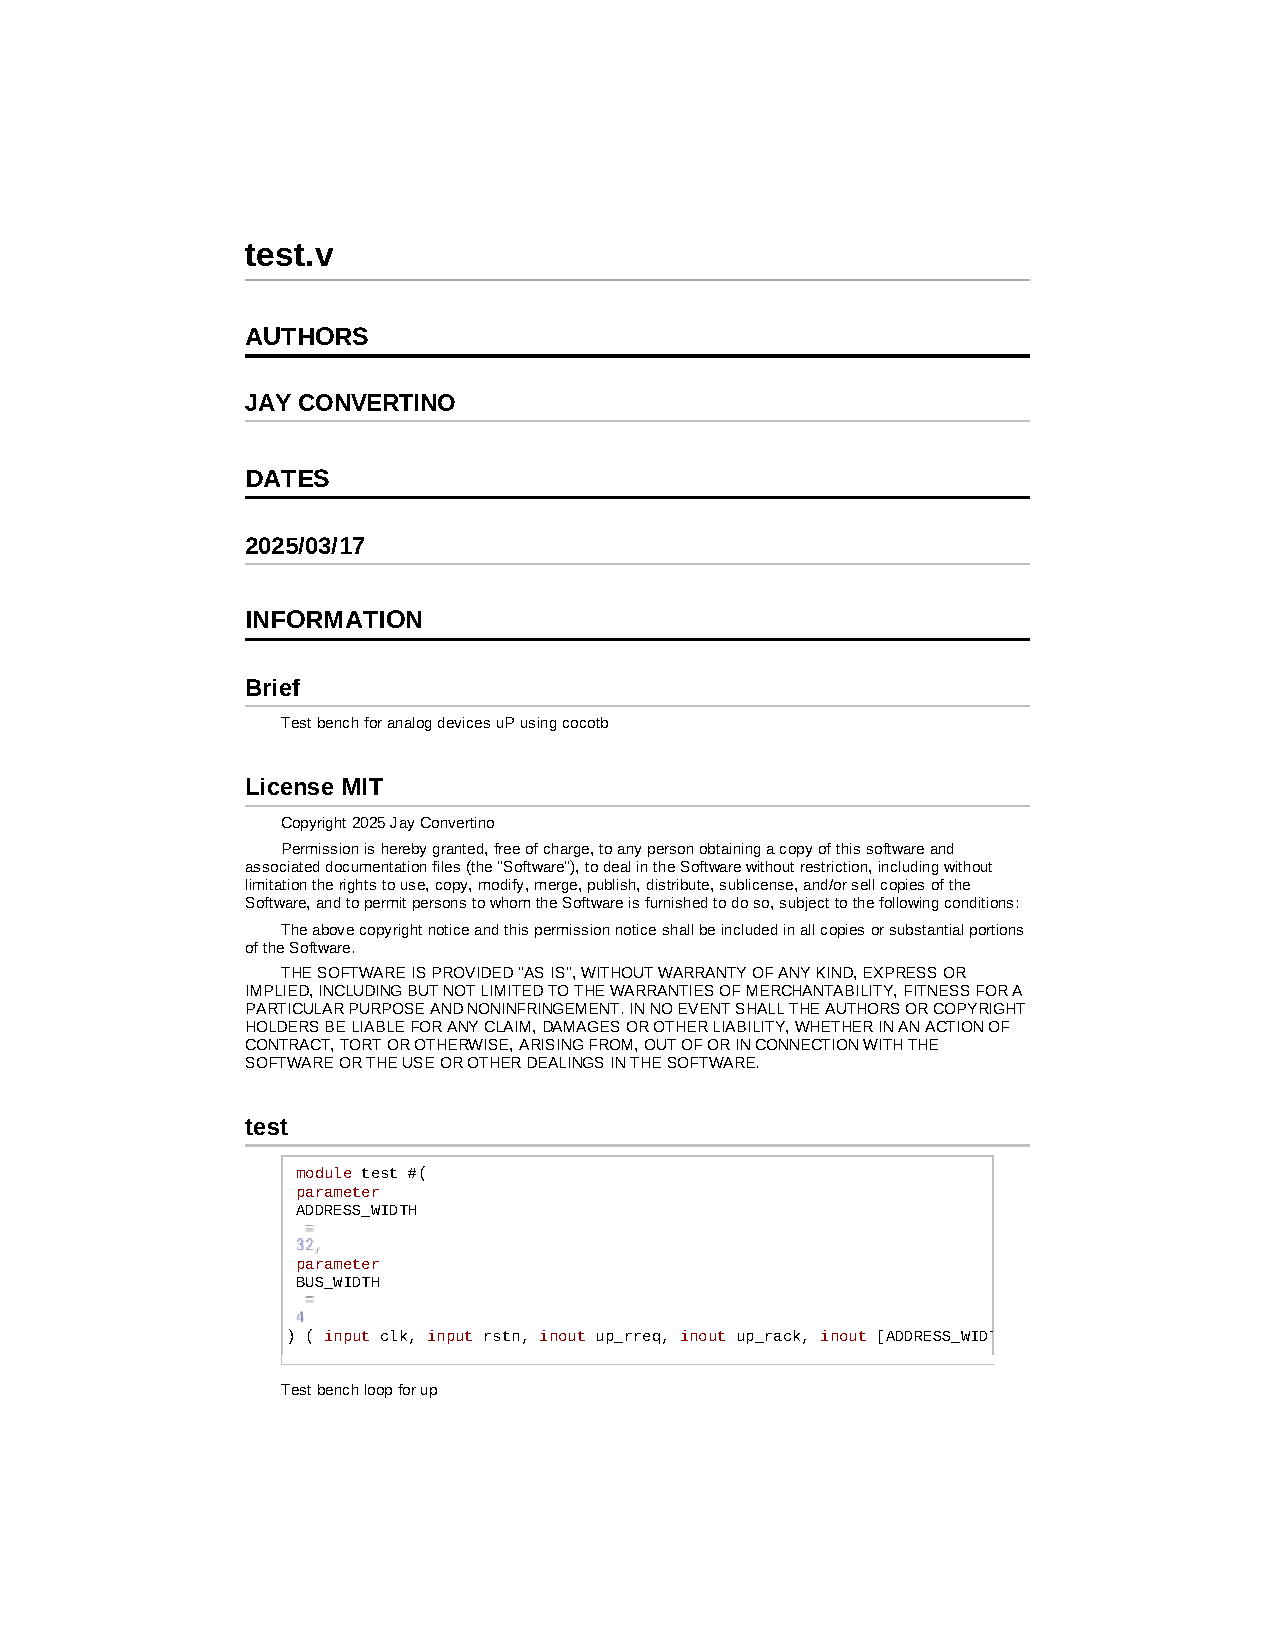
\includepdf[pages=-, addtotoc={1,subsection,1,test extension verilog,p1}, pagecommand={}]{files2_test-v.pdf}

\end{document}
